\documentclass{llncs}
\usepackage{amsmath}
\usepackage{upgreek}
\usepackage{dsfont}
\usepackage{mdframed}
%margin package
\usepackage[margin=1in,includefoot]{geometry}
%graphics packages
\usepackage{graphicx}
\usepackage{float}
%pseudocode packages
\usepackage{amsmath}
\usepackage{algorithm}
\usepackage[noend]{algpseudocode}
%hyperlinks
\usepackage{hyperref}

\begin{document}

\title{ON THE SEQUENCE TO SEQUENCE MODEL FOR DIALOGUE SYSTEMS}

\author{Wilbert Pumacay}

\institute{Catholic University San Pablo\\
\email{wilbert.pumacay@ucsp.edu.pe}}

\maketitle

\begin{abstract}

Sequence to sequence models are the referent in machine translation. Because of its success it has been used in some other tasks, in particular dialogue systems. This paper focuses on reproducing the results of the ``Neural Conversational Model'' by Oriol Vinyals and Quoc Le, analyzing some of its upsides and downsides, as well as analyzing some ways the model can be improved.

\keywords{Recurrent Neural networks, Sequence to sequence, dialogue systems}

\end{abstract}

\section{Introduction}

Over the last decade, the raise of deep learning has shift the paradigm by which we tackle various tasks from engineering features. We now let our models learn the representations themselves by providing sufficient data, computing power and good architectures. One of the areas this shift has made the more impact is in Natural Language Processing ( NLP ), having now good models for tasks such as machine translation, text summarization, language modelling, etc. .
\\
\\
In the case of machine translation, the state of the art model used is the Sequence to Sequence model \cite{seq2seq}, which makes great use of Recurrent neural network architectures, being the basic idea to compress a given sequence into a context vector, which gives the general idea of the sequence, and then use this vector to generate a resulting sequence that is the translation of the input sequence.
\\
\\
It seems quite natural that this idea of compressing the meaning of a sequence into a representation and then using it to create some sequence can be useful in the context of dialogue systems, where we can compress the meaning of a question into a vector and then generate a response in regards of this context.
\\
\\
As we will see, this approach brings some basic results that are not comparable with our expectations of a dialogue system, but by running into this problems we can see where the model can be improved or what characteristics should a better model have in order to tackle this problem.

\section{Main concepts}

Before we run into the model itself, let us analyze some concepts that are used in the context of deep learning and NLP, mainly the required background to understand the model.

\subsection{Recurrent Neural Networks}

When dealing with sequences of data the way-to-go approach is using Recurrent Neural Networks (RNNs). Using these, we are not constrained to the models in which the inputs should be fixed-length, which in the context of word sequences in would mean to construct a big sparse representation of the whole sequence into a single vector. Instead, we can pass our input in chunks of fixed size, each chunk being a word in some vector representation.


\begin{figure}[H]
    \centering
    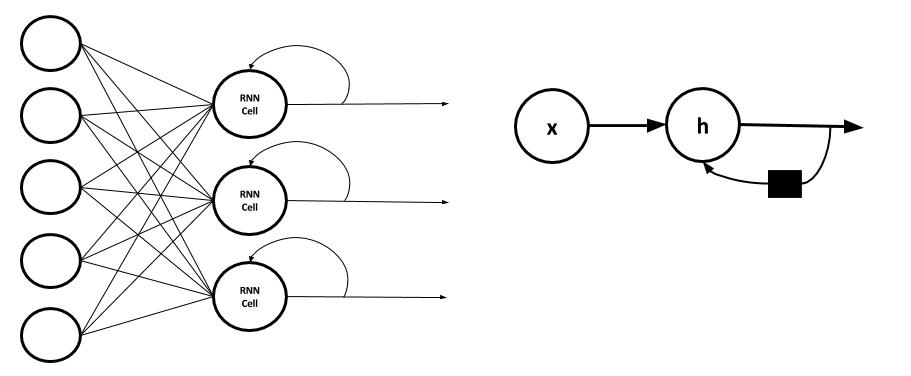
\includegraphics[scale=0.4]{../_img/img_rnn_folded.jpg}
    \caption{(Left) Single Layer RNN. (Right) Compressed representation of the RNN to the left}
    \label{fig:img_rnn_folded}
\end{figure}

In the figure above you can see that there is a feedback loop connection the output of the RNN cell to itself. This is the esscence of the RNN, using the previous output ( or state if connecting just before the output ) in the next computation step.

The computation made by this RNN can be described by this equation :

\begin{equation}
h_{t} = f( x_{t}, h_{t-1} ) = tanh( W_{x} x_{t} + W_{h} h_{t-1} + b )
\end{equation}

Were $W_{x}$ and $W_{h}$ are the weights of the matrix; the first one to add the contribution of the input at time step $t$, and the second to add the contribution of the previous hidden state.
\\
\\
It is ussually better to think of the RNN in an unfolded form, in which we see all the computations made through time. Because of the recurrence, we have a structure similar to the one shown in the figure below.

\begin{figure}[H]
    \centering
    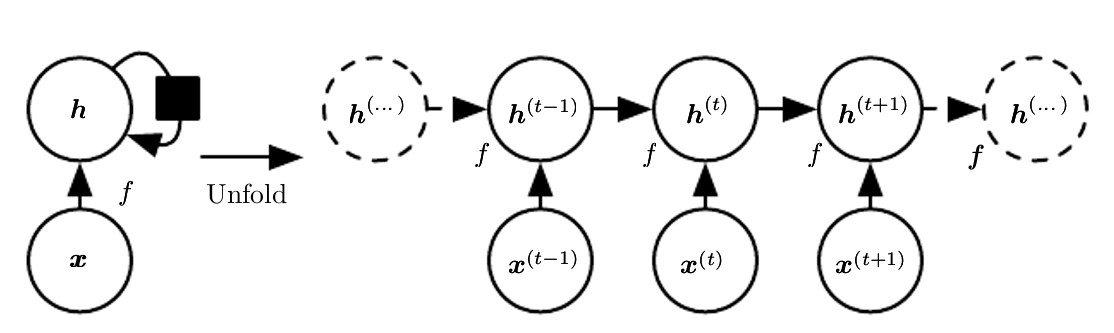
\includegraphics[scale=0.4]{../_img/img_dlb_rnnUnfolded.jpg}
    \caption{(Left) Single Layer RNN in folded form. (Right) Unfolded RNN though time. Figure from the Deep Learning book \cite{deeplearningbook}}
    \label{fig:img_dlb_rnnUnfolded}
\end{figure}

This helps when dealing with training, because we can think of a single layer RNN as a sequence of feedforward neural networks, with the number of hidden layers being equal to the number of time steps used in the computation. This yields the \textbf{ Backpropagation through time } algorithm, in which we compute the gradients through each time step having the weights $W_{x}$ and $W_{h}$ fixed through the whole computation.

\subsection{RNN Cells}

Because of the inherited recurrences in the computations in an RNN, we have to deal with 2 main problems when computing the gradients : exploding gradients and vanishing gradients. This arises because of the resulting recurrent multiplications in the gradient computation, having matrix exponentiations to some exponents, that in cases where the eigen values are greater than 1, the gradients explode, and in cases where the eigen values are less than 1, the gradients vanish.
\\
\\
To fix the first problem, a solution would be to use \textbf{Gradient clipping}, by which we normalize the gradient up to some magnitude if surpasses a certain threhsold. To fix the second problem, one solution is to use \textbf{Gated cells}, which basically modify the computations of the vanilla RNN cells and make the unfolded computations go from series of multiplications to series of summations.

\subsubsection{LSTM cell}~\\

The LSTM cell, first introduced by Hochreiter and Schmidhuber \cite{LSTM}, consists of gates in the computation that allow to pass certain signal in some degree. These gates consist of sigmoid cells that act like valves, having the result of the hidden state, cell state and input to the cell contribute in ertain levels to the next hidden state and cell state.
\\
\\
The following figure shows one of this cell.

\begin{figure}[H]
    \centering
    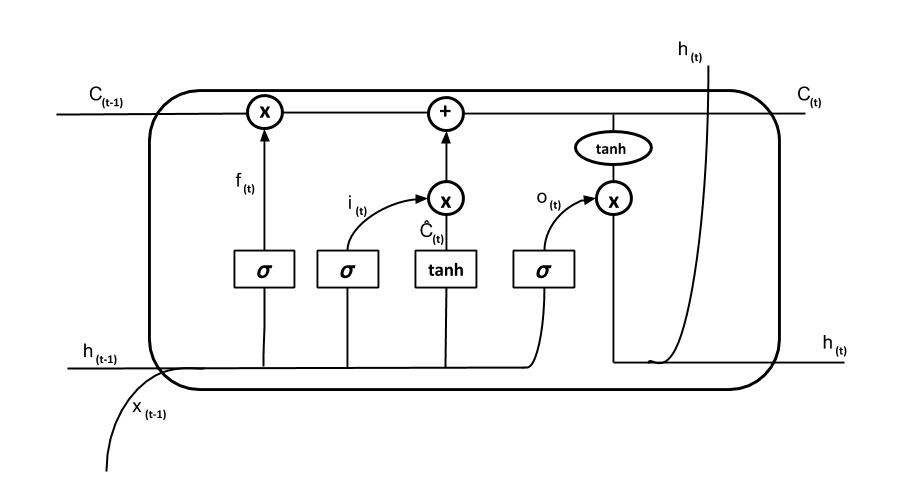
\includegraphics[scale=0.4]{../_img/img_lstmcell.jpg}
    \caption{An LSTM cell, with its gates and input-output relations}
    \label{fig:img_lstmcell}
\end{figure}

As you can see, there are three sigmoid gates. These are called \textbf{forget (f)}, \textbf{input (i)} and \textbf{output (o)} gates. The complete computation made by this cell can be enclosed in the following set of equations :

\begin{equation}
    \begin{gathered}
    f_{t} = \sigma( W_{f} [ h_{t - 1}, x_{t} ] + b_{f} ) \\
    i_{t} = \sigma( W_{i} [ h_{t - 1}, x_{t} ] + b_{i} ) \\
    o_{t} = \sigma( W_{o} [ h_{t - 1}, x_{t} ] + b_{o} ) \\
    C^{'}_{t} = tanh( W_{c} [ h_{t-1}, x_{t} ] + b_{c} ) \\
    C_{t} = C_{t-1} * f_{t} + C^{'}_{t} * i_{t} \\
    h_{t} = tanh( C_{t} ) * o_{t}
    \end{gathered}
\end{equation}

\subsubsection{GRU cell}~\\

The GRU cell, introduced by Kyunghyun et al. \cite{GRU}, is a variation of the LSTM cell that has the advantage of being simpler to compute and implement.
\\
\\
The following figure shows this cell :

\begin{figure}[H]
    \centering
    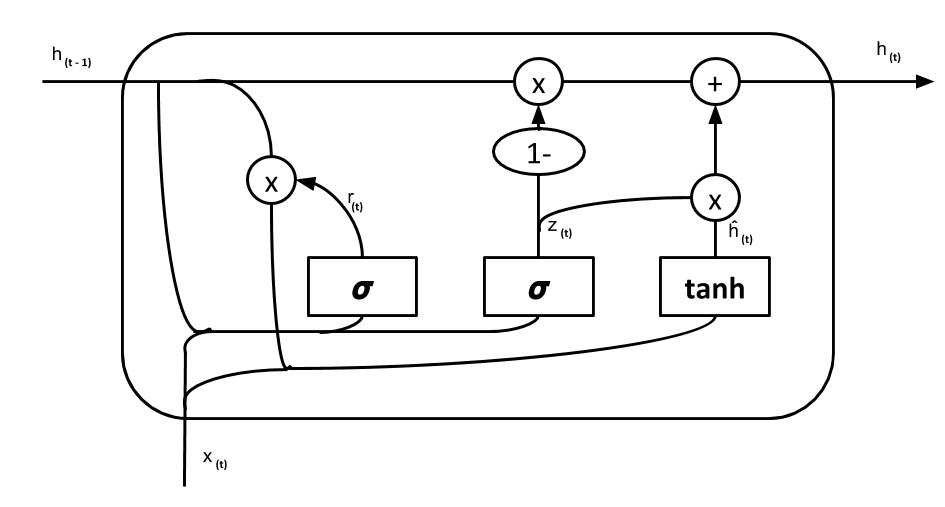
\includegraphics[scale=0.4]{../_img/img_grucell.jpg}
    \caption{A GRU cell, with its gates and input-output relations}
    \label{fig:img_grucell}
\end{figure}

The amount of computation is reduced, as it only uses 2 gates : update and reset. Its complete computation is described in the following set of equations :

\begin{equation}
    \begin{gathered}
    z_{t} = \sigma( W_{z} [ h_{t - 1}, x_{t} ] ) \\
    r_{t} = \sigma( W_{r} [ h_{t - 1}, x_{t} ] ) \\
    h^{'}_{t} = tanh( W_{h} [ r_{t} * h_{t-1}, x_{t} ] ) \\
    h_{t} = ( 1 - z_{t} ) * h_{t - 1} + z_{t} * h^{'}_{t}
    \end{gathered}
\end{equation}

\subsection{Word embeddings}

Word embeddings are a vector representation of words by which we represent each word in a vocabulary by a fixed-size vector in a high dimensional space. They key idea behind this vectors is that words that are used in similar context or mean something similar are close in this high dimensional space.

We can get these embeddings by training a neural network in an unsupervised way, by making the outputs of the network to be the probability of a word appearing in the context of another word, for a whole corpus of text. By maximizing this probability, we get the embeddings in the weights of this neural network, getting an embeddings matrix from which we can look-up the single embeddings related to each word.

These vectors are the inputs to various architectures used in NLP, being the inputs to our sequence to sequence model, as we will show in the following section.

\subsection{Sequence to sequence model}

The sequence to sequence model, introduced by Sutskever et al. \cite{seq2seq}, consists of an architecture of two Recurrent Neural Networks. The first one is called \textbf{Encoder}, an it is in charge of converting an input sequence into a fixed size vector that represents the whole sequence. This context vector is then used by the second network called \textbf{Decoder} to generate an output sequence. This architecture is shown in the following figure.

\begin{figure}[H]
    \centering
    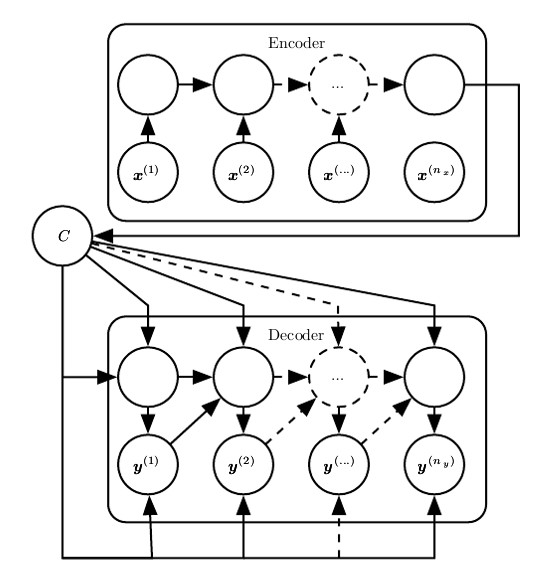
\includegraphics[scale=0.4]{../_img/img_dlb_encoderDecoder.jpg}
    \caption{The sequence to sequence architecture, taken from the Deep learning book \cite{deeplearningbook}}
    \label{fig:img_dlb_encoderDecoder}
\end{figure}

This model was first introduced in the context of generating sequences from sequences, like in machine translation. This model is adapted in our case to deal with dialog, by which the input is a question and the output the system's answer.

\section{Implementation}

We implemented the model using the Tensorflow framework and its sequence to sequence API. In the following sections we give some details of each piece that we implemented.

\subsection{Architecture}

We implemented the architecture studied in \cite{neuralConversation}, in which they used an encoder and a decoder using LSTM cells. The encoder inputs are of fixed length in time, so we accept a maximun number of input words to the encoder. The same applies for the decoder.

The following figure shows the overall architecture.

\begin{figure}[H]
    \centering
    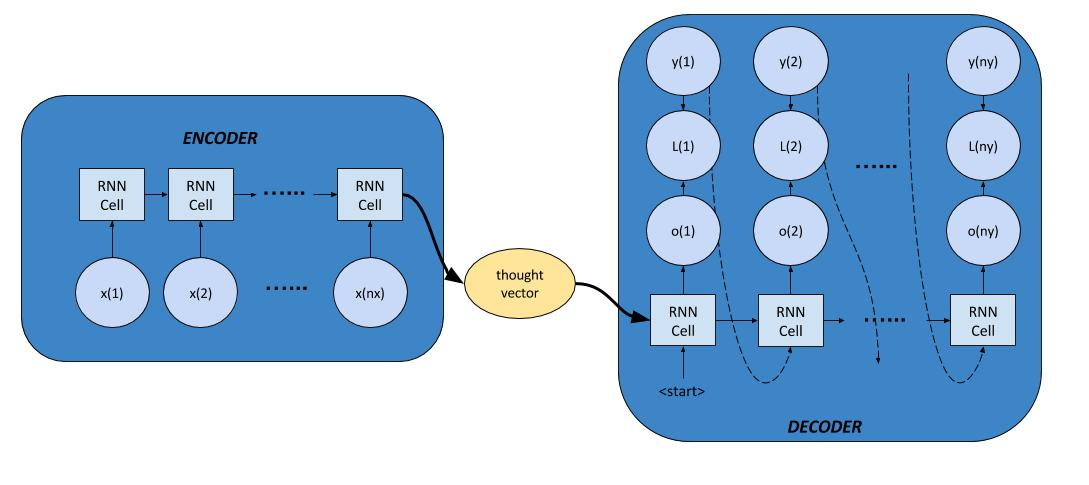
\includegraphics[scale=0.4]{../_img/img_seq2seq.jpg}
    \caption{The architecture implemented}
    \label{fig:img_seq2seq}
\end{figure}

\subsection{Sequence generation}

As we explained earlier, our models makes use of word vectors to represent the encoder input, as well as the decoder inputs. But instead of transforming a whole sequence into a sequence of vectors of fixed size, the API we used allows us to lookup the word vectors from the embeddings matrix by just giving a single lookup id, which are the unique ids in the dictionary we built from our dataset. This is shown in the following figure.

\begin{figure}[H]
    \centering
    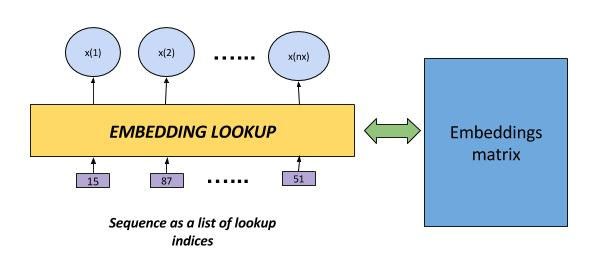
\includegraphics[scale=0.4]{../_img/img_embeddingLookup.jpg}
    \caption{Embedding lookup}
    \label{fig:img_embeddingLookup}
\end{figure}

Some input sequences may be shorter than the size specified earlier. In these situations we feed the encoder a padded version of these sequences, by adding a padding token until we fill the input size required by the encoder, like shown in the figure below.

\begin{figure}[H]
    \centering
    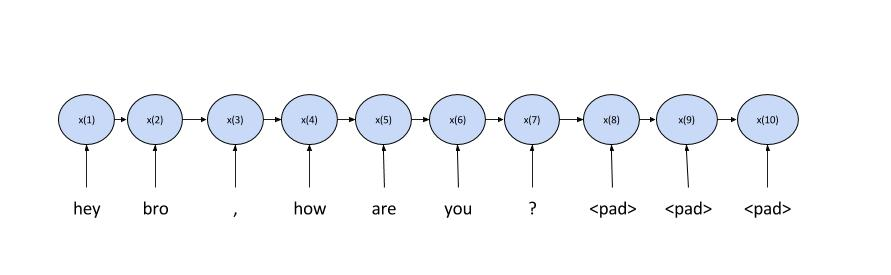
\includegraphics[scale=0.5]{../_img/img_encoderPadding.jpg}
    \caption{Padding of input sequences}
    \label{fig:img_encoderPadding}
\end{figure}

\subsection{Operation modes}

Depending of whether we are in training or test mode ( inference mode ), we wire the decoder differently.
\\
\\
In training mode, we connect the target outputs ( the answer sequences of our training examples ) to the decoder inputs in the next time step. This technique is called teacher forcing.
\\
\\
In the testing case, we feed the actual predicted words as the inputs to the decoder in the next time step. This is done because in test mode the model is required to generate the output sequence on its own.

\subsection{Dataset}

We used the Cornell Movie-Dialogs dataset, which consists of a set of dialogues taken from various movies. We parsed this data in various step to get the vocabulary and the question-answers sequences as ids, in order to get the batches we would feed into our model for training.

\section{Experimental results}

We trained our model with the following configuration :

\begin{table}[ht]
\centering
\begin{center}
\begin{tabular}{l@{\quad}rl}
\hline
\multicolumn{1}{l}{\rule{0pt}{12pt}
                   Parameter}&\multicolumn{2}{l}{Value}\\[2pt]
\hline\rule{0pt}{12pt}
Cell used                           &  GRU& \\
Number of layers                    &  2& \\
Number of hidden units per layer    &  512& \\
Input sequence length               &  20& \\
Output sequence length              &  20& \\
Attention                           &  No& \\
Dropout                             &  0.9& \\
Embeddings size                     &  100& \\
Softmax samples                     &  512& \\
Learning rate                       &  0.002& \\
Batch size                          &  256& \\
Epochs                              &  50& \\[2pt]
\hline
\end{tabular}
\caption{Model configuration}
\end{center}
\end{table}

We left the model training for approximately 8 hours in a computer with an i7 CPU and a GTX 750ti GPU, and got the following answers to some questions we feed into the model in test time :

\begin{figure}[H]
    \centering
    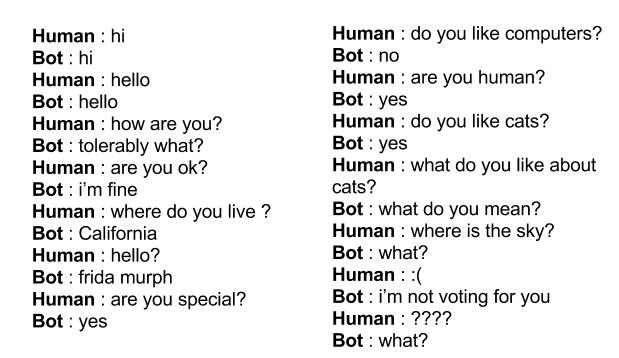
\includegraphics[scale=0.5]{../_img/img_chatbotLogs.jpg}
    \caption{Responses of the chatbot in test time}
    \label{fig:img_chatbotLogs}
\end{figure}

As you can see, the bot can generate sequences that have some meaning. At the start of a training session, if tested separately, we could see that the answers were erratic, saying nonsenses in all the cases. After training it could recognize when to stop ( it generated the stop token appropiately ) and generated some meaningful responses.
\\
\\
The problem of course is that the model breaks quite easily, as you can see in one of the cases where we asked `hello?' instead of `hello' and got totally different answers. 
\\
\\
It also has only responses to single questions, it fails to generate responses based on several steps before, which is natural in a conversation.

\section{Some analysis}

Based on how the model works and some insight from various sources, we can get some conclusions for the results we got with this model.
\\
\subsection{Compression coherence}

First, we got the issue of generating various different answers for some questions that are basically the same, as in the case when we said `hello?' instead of `hello'.
Our model should be robust enough to get these cases right. We call this feature \textbf{Compression coherence}, because it is related to the fact that when compressing ( encoder step ) into a thought vector, for similar questions we should get compressions that are similar or close in the high dimensional space of the thought vector.

\begin{figure}[H]
    \centering
    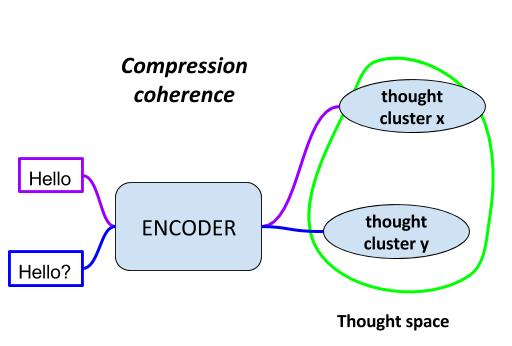
\includegraphics[scale=0.5]{../_img/img_compressionCoherence.jpg}
    \caption{Compression coherence}
    \label{fig:img_compressionCoherence}
\end{figure}

In our case, our results suggest that we are breaking this feature, and after training the encoder weights are acting quite erratically when compressing the sequences. I try to visualize this as in the case of the gradient clipping problem; if we are near a high hill then the gradients explode and get us very far from the point we were. Similarly, the encoder is throwing the vectors into sections of the \textbf{thought space} that are very far away for inputs that should be similar.
\\
\\
This also suggests that our training policies should account into making sure that the weights keep compression coherence all the time. We might try changing the optimization procedure to optimize for this metric, as well as trying to mimic the questions responses. One way I thought how the loss would be is the following :

\begin{equation}
J = \frac{1}{m} \sum^{m}_{i} \sum^{m}_{j} 1[h_{coh}( x^{(i)}, x^{(j)}) ] * ( encode( x^{(i)} ) - encode( x^{(j)} ) )
\end{equation}

Where $h_{coh}$ is a function that returns true or false if two sequences $x^{(i)}$ and $x^{(j)}$ belong to the same context; and $encode$ is just the encoder function.

This could be combined with the regular loss, in some way similar to regularization, to make sure that we keep this property.

\subsection{Thought space arbitration}

After listening to a talk of Ian Goodfellow, he gave an analogy as to how to think of the weights of a RNN. He suggested that the weights of an RNN are quite similar to the way we learn to perform a `task', by task being, for example, learning how to ride a bicycle. On the other hand, this is quite different to the ways we learn some other stuff, like, talking in a meaningful way.
\\
\\
In regards of this, one can think that there is a piece missing into the pipeline. Neural networks can be thought as compressing machines, were in the context of learning the representation we are compressing some knowledge into some lower dimensional space without loss of information. Then, what me are missing is what to do with this information.
\\
\\
The sequence to sequence model shows a case in which we directly used this compression into a decompression in the next step of the pipeline. There is no mechanism in between to handle some extra storing-retrieval of information. We called this mechanism an \textbf{arbitration mechanism}.
\\
\\
We think of this feature as a way to handle the data in this space. It is like a machine that knows how to store, how to organize and how to retrieve information from this thought space.
\\
\\ 
So, in regards of dialogue systems, some kind of arbitration would be helpful when trying to deal with more natural conversations.

\section{Performance metrics}

We already suggested that we could optimize for compression coherence. This could be used as a metric to test the performance of our system. What is more, this would ensure that for mispellings our system would not break.
\\
\\
We could also think of this in the decoder side, where if we sample from the thought space with two thought vectors that are close to each other, we should get responses that are coherent. We could also keep this metric in control to allow wild behavior when sampling from this space.
\\
\\
Apart from this, when trying to measure the performance of such a system, we are basically designing test cases for a subset of a turing test. One way we could achieve this is by grouping the testing data into parts that serve as a unit test for some features that the system should keep in check to pass the test. We basically have to group our test data in a way that we can have good test cases.
\\
\\
In this context, we could have tests for ensuring the system does not generate responses that may be inappropiate in some context ( racism for example ).
\\
\\
We can also make tests to ensure that the some features of the system are present or enhanced, like being supporting towards the user, etc..
\\
\\
With arbitration this could be achieved by the means of controlling the thought space properly. 

\section{Conclusions}

By studying the sequence to sequence model applied to the context of a dialogue system, we saw that it can generate quite meaningful answers in some cases. Even though the modest results, as suggested by the original authors, it is quite interesting that by using a pure data driven approach the model can learn quite useful representation to be used in a conversation. 
\\
\\
We can also conclude that there is some extra mechanism needed in between the encoding and decoding steps. This would help to handle more general scenarios in the conversation. 
\\
\\
We also saw that we may try to optimize for some other metrics that would ensure some robustness in the model, being this the compression and decompression coherence.


\begin{thebibliography}{9}

\bibitem{LSTM}
Hochreiter, Sepp and Schmidhuber, Jürgen.\\
\textit{Long Short-term Memory}\\
Neural computation, 1997.\\

\bibitem{GRU}
Kyunghyun et al.\\
\textit{Learning Phrase Representations using RNN Encoder-Decoder for Statistical Machine Translation}\\
Proceedings of the 2014 Conference on Empirical Methods in Natural Language Processing (EMNLP), 2014.\\

\bibitem{seq2seq}
Ilya Sutskever, Oriol Vinyals, Quoc V. Le.\\
\textit{ Sequence to Sequence Learning with Neural Networks}\\
NIPS'14 Proceedings of the 27th International Conference on Neural Information Processing Systems - Volume 2, 2014 \\

\bibitem{neuralConversation}
Oriol Vinyals, Quoc Le.\\
\textit{A neural conversational model}\\
ICML Deep Learning Workshop, 2015 \\

\bibitem{deeplearningbook}
Ian Goodfellow, Yoshua Bengio and Aaron Courville.\\
\textit{Deep learning}\\
MIT Press, 2016 \\

\bibitem{tensorflow}
Mart\'{\i}n~Abadi and
    Ashish~Agarwal and
    Paul~Barham and
    Eugene~Brevdo and
    Zhifeng~Chen and
    Craig~Citro and
    Greg~S.~Corrado and
    Andy~Davis and
    Jeffrey~Dean and
    Matthieu~Devin and
    Sanjay~Ghemawat and
    Ian~Goodfellow and
    Andrew~Harp and
    Geoffrey~Irving and
    Michael~Isard and
    Yangqing Jia and
    Rafal~Jozefowicz and
    Lukasz~Kaiser and
    Manjunath~Kudlur and
    Josh~Levenberg and
    Dan~Man\'{e} and
    Rajat~Monga and
    Sherry~Moore and
    Derek~Murray and
    Chris~Olah and
    Mike~Schuster and
    Jonathon~Shlens and
    Benoit~Steiner and
    Ilya~Sutskever and
    Kunal~Talwar and
    Paul~Tucker and
    Vincent~Vanhoucke and
    Vijay~Vasudevan and
    Fernanda~Vi\'{e}gas and
    Oriol~Vinyals and
    Pete~Warden and
    Martin~Wattenberg and
    Martin~Wicke and
    Yuan~Yu and
    Xiaoqiang~Zheng\\
\textit{ TensorFlow: Large-Scale Machine Learning on Heterogeneous Systems }\\
2015 \\

\end{thebibliography}

\end{document}
